\section{eo\-Replacement$<$ EOT $>$ Class Template Reference}
\label{classeo_replacement}\index{eoReplacement@{eoReplacement}}
{\tt \#include $<$eo\-Replacement.h$>$}

Inheritance diagram for eo\-Replacement$<$ EOT $>$::\begin{figure}[H]
\begin{center}
\leavevmode
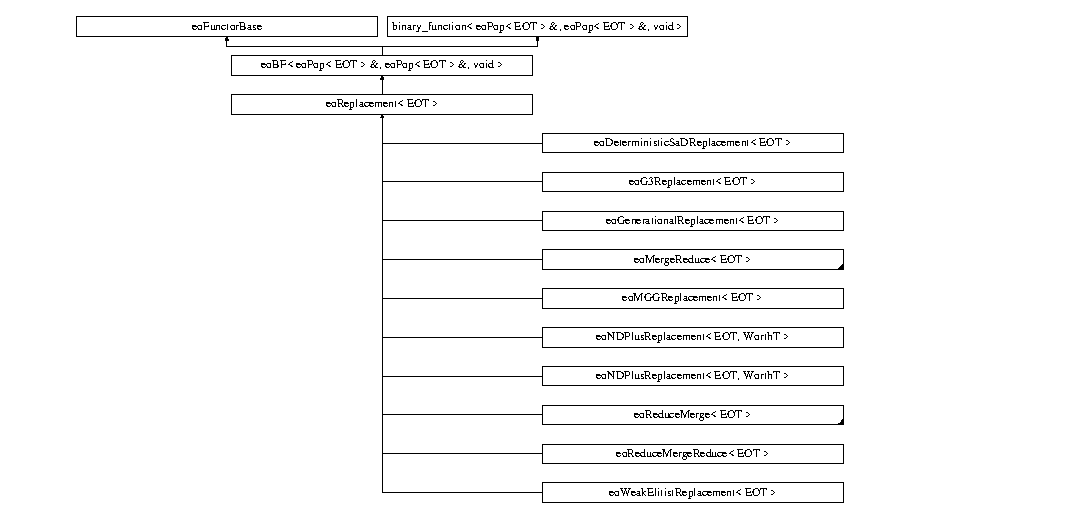
\includegraphics[height=6.5233cm]{classeo_replacement}
\end{center}
\end{figure}


\subsection{Detailed Description}
\subsubsection*{template$<$class EOT$>$ class eo\-Replacement$<$ EOT $>$}

NOTE: 2 {\bf eo\-Pop}{\rm (p.\,\pageref{classeo_pop})} as arguments the resulting population should be in the first argument (replace parents by offspring)! The second argument can contain any rubbish

--- The {\bf eo\-Merge\-Reduce}{\rm (p.\,\pageref{classeo_merge_reduce})}, combination of {\bf eo\-Merge}{\rm (p.\,\pageref{classeo_merge})} and {\bf eo\-Reduce}{\rm (p.\,\pageref{classeo_reduce})}, can be found in file {\bf eo\-Merge\-Reduce.h}{\rm (p.\,\pageref{eo_merge_reduce_8h})}

The {\bf eo\-Reduce\-Merge\-Reduce}{\rm (p.\,\pageref{classeo_reduce_merge_reduce})} that reduces the parents and the offspring, merges the 2 reduced populations, and eventually reduces that final population, can be found in {\bf eo\-Reduce\-Merge\-Reduce.h}{\rm (p.\,\pageref{eo_reduce_merge_reduce_8h})}

LOG --- Removed the const before first argument: though it makes too many classes with the same interface, it allows to minimize the number of actual copies by choosing the right destination I also removed the enforced \char`\"{}swap\char`\"{} in the eo\-Easy\-Algo and hence the generational replacement gets a class of its own that only does the swap (instead of the eo\-No\-Replacement that did nothing, relying on the algo to swap popualtions). MS 12/12/2000

\begin{Desc}
\item[See also:]{\bf eo\-Merge}{\rm (p.\,\pageref{classeo_merge})}, {\bf eo\-Reduce}{\rm (p.\,\pageref{classeo_reduce})}, {\bf eo\-Merge\-Reduce}{\rm (p.\,\pageref{classeo_merge_reduce})}, {\bf eo\-Reduce\-Merge}{\rm (p.\,\pageref{classeo_reduce_merge})}\end{Desc}
eo\-Replacement, base (pure abstract) class {\bf eo\-Generational\-Replacement}{\rm (p.\,\pageref{classeo_generational_replacement})}, as it says ... {\bf eo\-Weak\-Elitist\-Replacement}{\rm (p.\,\pageref{classeo_weak_elitist_replacement})} a wrapper to add elitism 



Definition at line 77 of file eo\-Replacement.h.

The documentation for this class was generated from the following file:\begin{CompactItemize}
\item 
eo\-Replacement.h\end{CompactItemize}
